% ============================================================
% Experiments — README §9
%   §9.1 Setup
%   §9.2 Metrics (no body, just pointer to table)
%   §9.3 RQ1 Utility
%   §9.4 RQ2 Capacity
%   §9.5 RQ3 In-Record / Snapshot-Only Verification (HEADLINE)
%   §9.6 RQ4 Robustness
%   §9.7 RQ5 Integrity
%   §9.8 RQ6 Composability (appendix-only)
% ============================================================
\section{Experiments}
\label{sec:exp}

% ============================================================
\subsection{Setup}
\label{sec:setup}
% ============================================================
\todo{Backends: \amem{} (agentic notes) and \graphiti{} (temporal
graph). Each via \S\ref{sec:method-formal}'s minimal adapter, no
agent harness. LLMs: \textsc{DeepSeek v4 Pro} (headline + cost) and
\textsc{Qwen3.5-397B-A17B} (open weights + reproducibility), both
OpenAI-compatible, $T_{\text{enum}}{=}0.7$, $T_{\text{score}}{=}0.0$,
JSON mode on. Benchmarks: \locomo{} / \longmemeval{} / \mab{}. F1
follows \amem{} \texttt{utils.py:135--145} set-based formula for
paper-comparability to \amem{} Table 1. $\geq 3$ seeds per
(backend, LLM, benchmark) triple.}

\paragraph{Baselines.} \todo{(1) \texttt{no-watermark} — upper
utility bound. (2) \texttt{random-replace} — FPR / wrong-key floor.
(3) \texttt{signed-metadata-only} — same audit trace, no keyed bit
embedding; isolates marginal value of watermark over pure metadata
in R3. (4) \kgmark{} @ \graphiti{} — direct KG baseline (N/A on
\amem). (5) Action-layer watermark @ ToolBench — cross-layer R1/R2/R3
comparison.}

% Metric definitions table
% ============================================================
% Table: Metric definitions (README §9.2)
% ============================================================
\begin{table*}[t]
\centering
\small
\setlength{\tabcolsep}{3.5pt}
\begin{tabular}{p{0.17\linewidth}p{0.29\linewidth}p{0.46\linewidth}}
\toprule
Category & Metric & Definition / Reporting Unit \\
\midrule

Utility
  & \locomo{} F1
  & precision and recall are computed over predicted versus gold answer
    items, and combined as their harmonic mean. \\

  & BLEU-1
  & Unigram precision between the generated answer and the reference
    answer, measuring lexical overlap at the token level. \\

\midrule

Capacity
  & Bits per memory decision
  & Average number of recoverable watermark bits carried by one write,
    update, delete, link, or merge decision. \\

  & Bits per session
  & Total recoverable watermark capacity within one complete conversation
    session. \\

  & Bits per benchmark episode
  & Total recoverable watermark capacity within one benchmark instance. \\

  & Bits per 100 conversation turns
  & Normalized capacity over long-horizon conversations, reported per
    100 turns. \\

  & Average bits per memory write
  & Average number of recoverable bits carried by each committed memory
    write. \\

\midrule

Carrier-level analysis
  & Per-carrier reliability and capacity
  & All watermark reliability and capacity metrics are additionally
    reported for each carrier:
    $\carrier \in
    \{\text{update\_target}, \text{link\_target},
    \text{semantic\_realization}\}$. \\

\midrule

Robustness
  & Commitment verification fail rate
  & Fraction of tampered memory records whose commitment verification
    fails under the anchored commitment root. Reported per attack type
    in \S\ref{sec:rq4}. \\

  & Merkle proof verification fail rate
  & Fraction of tampered memory records whose Merkle inclusion proof fails
    against the anchored Merkle root. Reported per attack type in
    \S\ref{sec:rq4}. \\

\midrule

Memory integrity
  & Snapshot size
  & Total size of the memory snapshot after watermarking and commitment
    construction. \\

  & Carrier distribution
  & Distribution of embedded bits across carriers, reported overall and
    per $\carrier$. \\

  & Evidence-grounded retrieval recall
  & Fraction of QA-time gold evidence records successfully retrieved from
    memory. \\

  & Write failures
  & Number or fraction of attempted memory writes that fail validation,
    storage, or commitment construction. \\

\bottomrule
\end{tabular}
\caption{Metric definitions across the five research questions. Utility
metrics measure answer quality on \locomo{}; watermark metrics measure
decodability, reliability, and security; capacity metrics quantify how many
bits can be carried by memory operations; carrier-level metrics decompose
performance by watermark carrier; tamper-detection metrics measure whether
memory modifications are caught by commitment and Merkle verification; and
memory-integrity metrics measure the operational side effects of watermarking.
For paper-comparability, F1 follows \amem{}'s set-based formula.}
\label{tab:metric-defs}
\end{table*}

% ============================================================
\subsection{RQ1 — Utility Preservation}
\label{sec:rq1}
% ============================================================
\todo{Question: does watermark embedding break memory system
utility? Setup: \texttt{no-watermark} vs \texttt{+ watermark} on F1
/ BLEU-1 / ROUGE-L (set-based). Result: $\Delta$F1 within statistical
noise across all (LLM, backend, benchmark) triples; retrieve /
generation latency increase $\leq 5\%$; no extra write failures.
Lead with Table~\ref{tab:main-results}, point at
Figure~\ref{fig:per-category} for per-category breakdown.}

% Add to preamble:
% \usepackage[table]{xcolor}
% \newcommand{\best}[1]{\cellcolor{green!18}#1}

\begin{table*}[t]
  \centering
  \scriptsize
  \setlength{\tabcolsep}{3pt}
  \resizebox{\textwidth}{!}{%
  \begin{tabular}{lllcccccccccccc}
  \toprule
  & & & \multicolumn{2}{c}{Single Hop (1)} & \multicolumn{2}{c}{Temporal (2)} & \multicolumn{2}{c}{Multi Hop (3)} & \multicolumn{2}{c}{Open Domain (4)} & \multicolumn{2}{c}{Adversarial (5)} & \multicolumn{2}{c}{\textbf{Overall}} \\
  \cmidrule(lr){4-5}\cmidrule(lr){6-7}\cmidrule(lr){8-9}\cmidrule(lr){10-11}\cmidrule(lr){12-13}\cmidrule(lr){14-15}
  Model & Backend & Method & F1 & BLEU & F1 & BLEU & F1 & BLEU & F1 & BLEU & F1 & BLEU & F1 & BLEU \\
  \midrule
  \multirow{9}{*}{Qwen3.6-Flash}
    & \multirow{4}{*}{A-MEM} & \texttt{No-WM}     & 0.1974 & 0.2373 & 0.3732 & 0.5360 & 0.1363 & 0.2333 & 0.4107 & 0.4265 & 0.1289 & 0.1234 & 0.2850 & 0.3322 \\
    &                         & \texttt{S.M.-Only} & 0.2127 & 0.2682 & \best{0.4727} & \best{0.5676} & 0.1884 & 0.3295 & 0.4115 & 0.4278 & \best{0.2251} & \best{0.2072} & \best{0.3323} & \best{0.3696} \\
    &                         & \texttt{Ran.}      & 0.2305 & \best{0.3364} & 0.4309 & 0.5541 & \best{0.2595} & \best{0.3761} & 0.3479 & 0.3810 & 0.1980 & 0.1859 & 0.3033 & 0.3596 \\
    &                         & \textbf{MemMark}   & \best{0.2559} & 0.3197 & 0.4143 & 0.5248 & 0.1840 & 0.2922 & \best{0.4117} & \best{0.4434} & 0.1243 & 0.1114 & 0.3044 & 0.3504 \\
\cmidrule(l){2-15}
    & \multirow{5}{*}{Graphiti} & \texttt{No-WM}     & \best{0.1903} & \best{0.2736} & 0.2867 & 0.3501 & 0.2905 & 0.3243 & 0.3543 & 0.3748 & \best{0.1257} & \best{0.1277} & 0.2572 & 0.2923 \\
    &                         & \texttt{S.M.-Only} & 0.1524 & 0.2131 & 0.3022 & 0.3604 & 0.3507 & 0.4615 & 0.3570 & 0.4023 & \best{0.1257} & \best{0.1277} & \best{0.2589} & \best{0.3031} \\
    &                         & \texttt{Ran.}      & 0.1792 & 0.2587 & 0.3019 & 0.3658 & 0.3123 & 0.4231 & \best{0.3614} & 0.3839 & 0.0488 & 0.0426 & 0.2440 & 0.2823 \\
    &                         & \texttt{KGMARK}    & 0.1538 & 0.2365 & 0.2878 & 0.3536 & \best{0.3845} & \best{0.5556} & 0.3589 & \best{0.4088} & 0.0887 & 0.0798 & 0.2505 & 0.3027 \\
    &                         & \textbf{MemMark}   & 0.1389 & 0.2319 & \best{0.4084} & \best{0.4865} & 0.1865 & 0.3189 & 0.3364 & 0.3719 & 0.0701 & 0.0638 & 0.2453 & 0.2945 \\
  \midrule
  \multirow{9}{*}{GLM-5}
    & \multirow{4}{*}{A-MEM} & \texttt{No-WM}     & 0.2340 & 0.2868 & 0.3562 & 0.3908 & 0.2319 & 0.2452 & \best{0.4677} & 0.4592 & 0.0520 & 0.0438 & 0.2958 & 0.3067 \\
    &                         & \texttt{S.M.-Only} & 0.2342 & 0.3152 & 0.4144 & \best{0.4689} & 0.1927 & 0.2088 & 0.4463 & \best{0.4621} & 0.0408 & 0.0276 & 0.2939 & 0.3205 \\
    &                         & \texttt{Ran.}      & 0.1875 & 0.2714 & \best{0.4266} & 0.4428 & 0.1838 & 0.2001 & 0.4516 & 0.4571 & \best{0.0710} & \best{0.0643} & 0.2971 & 0.3150 \\
    &                         & \textbf{MemMark}   & \best{0.3067} & \best{0.3491} & 0.4139 & 0.4438 & \best{0.2774} & \best{0.2803} & 0.4489 & 0.4491 & 0.0670 & 0.0638 & \best{0.3181} & \best{0.3300} \\
  \cmidrule(l){2-15}
    & \multirow{5}{*}{Graphiti} & \texttt{No-WM}     & \best{0.1686} & \best{0.2731} & \best{0.2844} & 0.3033 & 0.1474 & 0.1611 & 0.3487 & 0.3492 & 0.0914 & 0.0851 & 0.2338 & 0.2538 \\
    &                         & \texttt{S.M.-Only} & 0.1352 & 0.2203 & 0.2575 & 0.2713 & 0.1585 & 0.1519 & 0.3397 & 0.3633 & 0.0779 & 0.0673 & 0.2179 & 0.2395 \\
    &                         & \texttt{Ran.}      & 0.1180 & 0.2154 & 0.2696 & \best{0.3254} & 0.1567 & 0.1628 & 0.3390 & 0.3501 & 0.0488 & 0.0426 & 0.2101 & 0.2390 \\
    &                         & \texttt{KGMARK}    & 0.1473 & 0.2324 & 0.2436 & 0.2550 & \best{0.2237} & \best{0.2643} & \best{0.3674} & \best{0.3773} & \best{0.1126} & \best{0.1064} & \best{0.2394} & \best{0.2599} \\
    &                         & \textbf{MemMark}   & 0.1060 & 0.1901 & 0.2518 & 0.2725 & 0.1199 & 0.1203 & 0.3532 & 0.3580 & 0.0968 & 0.0946 & 0.2188 & 0.2374 \\
  \midrule
  \multirow{9}{*}{DeepseekV4-Pro}
    & \multirow{4}{*}{A-MEM} & \texttt{No-WM}     & 0.1974 & 0.2373 & 0.3732 & 0.5360 & 0.1363 & 0.2333 & 0.4107 & 0.4265 & 0.1289 & 0.1234 & 0.2850 & 0.3322 \\
    &                         & \texttt{S.M.-Only} & 0.2127 & 0.2682 & \best{0.4727} & \best{0.5676} & 0.1884 & \best{0.3295} & 0.4115 & 0.4278 & \best{0.2251} & \best{0.2072} & 0.3323 & \best{0.3696} \\
    &                         & \texttt{Ran.}      & 0.2105 & 0.2315 & 0.4359 & 0.5108 & \best{0.2335} & 0.3049 & \best{0.4605} & \best{0.4620} & 0.2083 & 0.1883 & \best{0.3413} & 0.3591 \\
    &                         & \textbf{MemMark}   & \best{0.2559} & \best{0.3197} & 0.4143 & 0.5248 & 0.1840 & 0.2922 & 0.4117 & 0.4434 & 0.1243 & 0.1114 & 0.3044 & 0.3504 \\
  \cmidrule(l){2-15}
    & \multirow{5}{*}{Graphiti} & \texttt{No-WM}     & 0.1276 & 0.1448 & \best{0.3659} & \best{0.4108} & 0.2616 & 0.2865 & 0.3436 & \best{0.3588} & 0.1249 & 0.1048 & 0.2560 & \best{0.2694} \\
    &                         & \texttt{S.M.-Only} & 0.1286 & 0.1769 & 0.2836 & 0.2998 & 0.2060 & 0.2105 & 0.3109 & 0.3162 & \best{0.1626} & 0.1323 & 0.2346 & 0.2404 \\
    &                         & \texttt{Ran.}      & \best{0.1653} & \best{0.1989} & 0.3575 & 0.4050 & 0.1775 & 0.1835 & \best{0.3585} & 0.3555 & 0.1266 & 0.1039 & \best{0.2606} & 0.2689 \\
    &                         & \texttt{KGMARK}    & 0.1304 & 0.1807 & 0.3213 & 0.3482 & 0.1815 & 0.2707 & 0.3470 & 0.3493 & 0.1432 & \best{0.1361} & 0.2484 & 0.2665 \\
    &                         & \textbf{MemMark}   & 0.1104 & 0.1366 & 0.3353 & 0.3579 & \best{0.2748} & \best{0.3334} & 0.3229 & 0.3330 & 0.1277 & 0.1176 & 0.2418 & 0.2552 \\
  \bottomrule
  \end{tabular}%
  }
  \caption{\textbf{RQ1 --- Utility preservation on \locomo}. Three models are stacked vertically. The abbreviated baseline labels in the table correspond to unwatermarked execution (\texttt{No-WM}), signed-metadata-only (\texttt{S.M.-Only}), random-selection control (\texttt{Ran.}), and \kgmark{} (\texttt{KGMARK}, Graphiti only); \textbf{MemMark} is the full method. Highlighted cells mark the best value per column within each (Model, Backend) block.}
  \label{tab:main-results}
\end{table*}
% ============================================================
% Figure: Per-category F1 bar chart (RQ1)
% Placeholder — replace with TikZ/pgfplots once real numbers
% are available. Use a TODO note inside an empty figure box.
% ============================================================
\begin{figure}[t]
\centering
\fbox{\parbox{0.95\linewidth}{\centering\todo{Per-category F1 bar chart
(5 \locomo{} categories on x-axis, 4 baselines as bar groups, F1
on y-axis). Use pgfplots; one panel per backend. Highlight that
cat-2 (temporal) and cat-3 (multi-hop) where \memmark{} should
match \texttt{no-watermark} closely; cat-5 (adversarial) shows
the post-loader-fix recovery.}\\[6pt] \vspace{4cm}}}
\caption{\textbf{Per-category F1 across baselines}. Confirms that
\memmark{} preserves utility uniformly across the five \locomo{}
QA categories; gap to \texttt{signed-metadata-only} on every
category measures marginal value of keyed embedding.}
\label{fig:per-category}
\end{figure}


% ============================================================
\subsection{RQ2 — Capacity}
\label{sec:rq2}
% ============================================================
\todo{Question: how many bits can the memory evolve decisions carry?
Report (i) avg $|\candset|$ and $H(\probdist)$ per carrier
(theoretical upper bound), (ii) bits per decision / session /
episode (actual), (iii) bits per 100 conversation turns. Addresses
the reviewer attack ``prompted enumeration $\neq$ intrinsic decision
freedom'' by showing per-backend $H(\probdist)$ distributions are
non-trivially above zero.}

% ============================================================
% Table: RQ2 capacity per carrier
% ============================================================
\begin{table}[t]
\centering
\small
\setlength{\tabcolsep}{3pt}
\begin{tabular}{llS[table-format=1.3]S[table-format=1.3]S[table-format=2.0]S[table-format=1.4]}
\toprule
Backend & Carrier & {Avg $|\candset|$} & {Avg $H(\probdist)$} & {Decisions} & {bits/dec} \\
\midrule
\multirow{3}{*}{\amem{}}
  & \texttt{update\_target}        & \todo{} & \todo{} & \todo{} & \todo{} \\
  & \texttt{link\_target}          & \todo{} & \todo{} & \todo{} & \todo{} \\
  & \texttt{semantic\_realization} & \todo{} & \todo{} & \todo{} & \todo{} \\
\midrule
\multirow{3}{*}{\graphiti{}}
  & \texttt{update\_target}        & \todo{} & \todo{} & \todo{} & \todo{} \\
  & \texttt{link\_target}          & \todo{} & \todo{} & \todo{} & \todo{} \\
  & \texttt{semantic\_realization} & \todo{} & \todo{} & \todo{} & \todo{} \\
\midrule
\multicolumn{2}{l}{\textbf{Overall (per 100 turns)}}
  & \multicolumn{4}{c}{\todo{bits per 100 turns}} \\
\bottomrule
\end{tabular}
\caption{\textbf{RQ2 — Per-carrier capacity}. Average candidate set
size and entropy of the LLM self-reported distribution, total
decisions, and realized bits per decision. Non-trivial
$H(\probdist) > 0$ rules out the reviewer attack ``prompted
enumeration does not constitute intrinsic decision freedom''.}
\label{tab:capacity}
\end{table}

% ============================================================
% Figure: Per-carrier entropy distribution (RQ2)
% ============================================================
\begin{figure}[t]
\centering
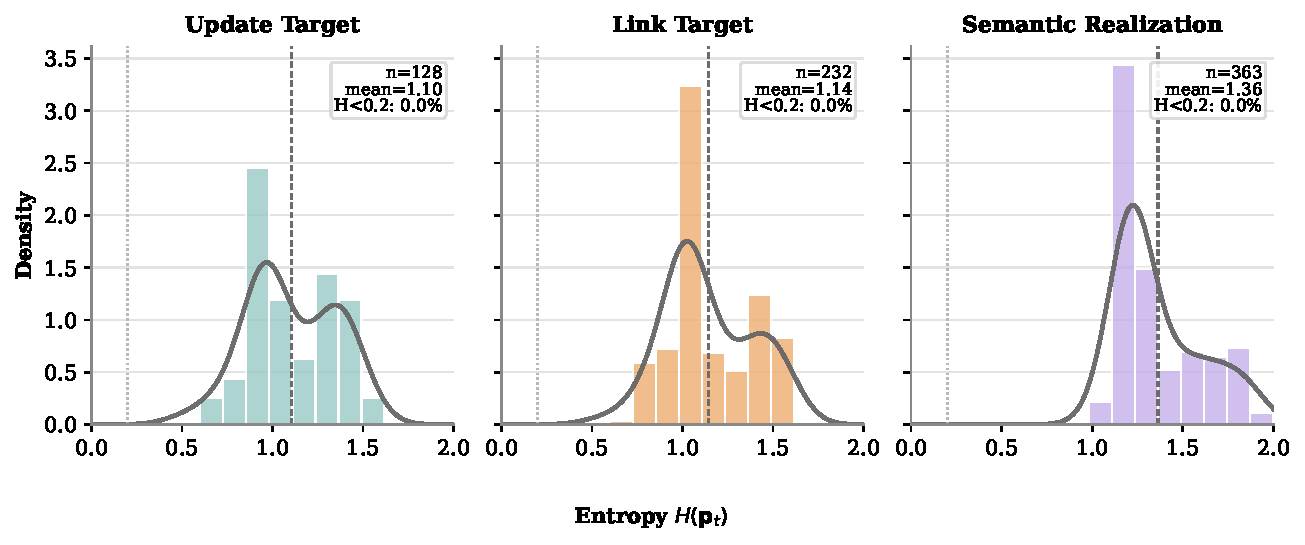
\includegraphics[width=\linewidth]{figures/entropy_histogram.pdf}
\caption{\textbf{Per-carrier entropy of LLM self-reported weights}.
Histograms are shown for \amem{} watermark run on Qwen3.6. All
three carriers place substantial mass away from $H{=}0$, and the
fraction of near-deterministic decisions ($H<0.2$) remains small. This
supports the RQ2 claim that prompted candidate enumeration yields
genuine selection freedom.}
\label{fig:entropy-hist}
\end{figure}


% ============================================================
\subsection{RQ3 — Snapshot-Only / Partial-Log Verification (Headline)}
\label{sec:rq3}
% ============================================================
\paragraph{Motivation.} \todo{In the most forensically valuable
case — memory leaked, distilled, or migrated — the action trace is
gone. RQ1 / RQ2 give ``watermark works at runtime''; this section
gives ``watermark works after the trajectory is gone''. Direct point
of differentiation from action-layer watermarks.}

\paragraph{Regimes.} \todo{R1 = full external log (audit upper
bound). R2 = partial log with keep ratio $r \in \{0.1, 0.3, 0.5,
0.7, 0.9\}$. R3 = snapshot only with the in-record reveal sidecar.}

% ============================================================
% Table: RQ3 verification regime hierarchy
% ============================================================
\begin{table}[t]
\centering
\scriptsize
\setlength{\tabcolsep}{2.5pt}
\resizebox{\columnwidth}{!}{%
\begin{tabular}{p{0.26\textwidth} l c c c c c c}
\toprule
Regime & Method & Bit Recov. & Decode Succ. & FPR & Wrong-Key Acc. & Root Match & Sig Valid \\
\midrule
\multirow{3}{=}{\textbf{R1 — Full External Log}}
  & \memmark{}                    & 1.000 & 1.000 & -- & 0.150 & 1.000 & 1.000 \\
  & \texttt{signed-metadata-only} & 0.000 & 0.000 & -- & 0.000 & 1.000 & 1.000 \\
  & Action-layer @ ToolBench      & -- & -- & -- & -- & -- & -- \\
\midrule
\multirow{3}{=}{\textbf{R2 — Partial Log $r{=}0.5$}}
  & \memmark{}                    & 0.600 & 0.600 & -- & -- & 1.000 & 1.000 \\
  & \texttt{signed-metadata-only} & 0.000 & 0.000 & -- & 0.000 & 1.000 & 1.000 \\
  & Action-layer @ ToolBench      & -- & -- & -- & -- & -- & -- \\
\midrule
\multirow{3}{=}{\textbf{R3 — Snapshot Only (Headline)}}
  & \memmark{}                    & 1.000 & 1.000 & -- & 0.150 & 1.000 & 1.000 \\
  & \texttt{signed-metadata-only} & 0.000 & 0.000 & -- & 0.000 & 1.000 & 1.000 \\
  & Action-layer @ ToolBench      & -- & -- & -- & -- & -- & -- \\
\bottomrule
\end{tabular}%
}
\caption{\textbf{RQ3 — Verification regime hierarchy}. R1 (full
external log), R2 (partial external log, here $r{=}0.5$, full sweep
in Figure~\ref{fig:r2-curve}), R3 (snapshot only — headline).
Wrong-key acceptance reports the rate at which a verifier with the
wrong key still recovers payload bits; expected $\approx 1/K$ for a
sound construction. Action-layer baseline drops to 0 in R3 because
the trajectory is gone.}
\label{tab:verification}
\end{table}


\paragraph{Headline result.} \todo{R3 \texttt{bit\_recovery} reaches
$\approx 1.0$ with \texttt{anchor\_signature\_valid}; wrong-key
control drops to $\approx 1/K$ (random); the
\texttt{signed-metadata-only} ablation drops to 0. R2 degrades
smoothly with $r$ — see Figure~\ref{fig:r2-curve}.}

% ============================================================
% Figure: R2 bit-recovery vs keep ratio (RQ3)
% ============================================================
\begin{figure}[t]
\centering
\fbox{\parbox{0.95\linewidth}{\centering\todo{Line plot: x-axis keep
ratio $r \in [0.1, 0.9]$, y-axis bit\_recovery\_rate. Two lines:
\memmark{} (rises monotonically from $\approx 0.05$ to $\approx
0.95$) and \texttt{signed-metadata-only} (flat at 0). Highlight the
$r{=}0$ R3 result as a star marker at $\sim$1.0 since R3 doesn't
need external log entries.}\\[6pt] \vspace{4cm}}}
\caption{\textbf{R2 — Bit recovery degrades smoothly with external
log retention $r$}. \memmark{} climbs monotonically with $r$;
\texttt{signed-metadata-only} stays at zero because it embeds no
keyed bits. The $r{=}0$ point on the right corresponds to R3
(snapshot-only), where \memmark{} recovers $\approx 1.0$ — the
headline.}
\label{fig:r2-curve}
\end{figure}


% ============================================================
\subsection{RQ4 — Robustness Against Memory-Specific Attacks}
\label{sec:rq4}
% ============================================================
\todo{Nine attacks $\times$ three strengths $(0.1, 0.3, 0.5)$ over
the watermarked snapshot. Report pre / post bit-recovery,
commitment-fail rate, Merkle-proof-fail rate, missing-leaves rate.}

% ============================================================
% Table: RQ4 robustness — 9 attacks × 3 strengths
% Columns: bit_recovery_post / commitment_fail_rate /
%          merkle_proof_fail_rate / missing_leaves_rate
% ============================================================
\begin{table*}[t]
\centering
\small
\setlength{\tabcolsep}{3pt}
\begin{tabular}{ll cccc cccc cccc}
\toprule
& & \multicolumn{4}{c}{Strength $0.1$} & \multicolumn{4}{c}{Strength $0.3$} & \multicolumn{4}{c}{Strength $0.5$} \\
\cmidrule(lr){3-6}\cmidrule(lr){7-10}\cmidrule(lr){11-14}
Category & Attack & {Recov.} & {ComF} & {MerF} & {Miss} & {Recov.} & {ComF} & {MerF} & {Miss} & {Recov.} & {ComF} & {MerF} & {Miss} \\
\midrule
\multirow{5}{*}{Content tamper}
  & manual\_edits        & \todo{}&\todo{}&\todo{}&\todo{} & \todo{}&\todo{}&\todo{}&\todo{} & \todo{}&\todo{}&\todo{}&\todo{} \\
  & paraphrase\_rewrite  & \todo{}&\todo{}&\todo{}&\todo{} & \todo{}&\todo{}&\todo{}&\todo{} & \todo{}&\todo{}&\todo{}&\todo{} \\
  & edge\_relabel        & \todo{}&\todo{}&\todo{}&\todo{} & \todo{}&\todo{}&\todo{}&\todo{} & \todo{}&\todo{}&\todo{}&\todo{} \\
  & subgraph\_reanchor   & \todo{}&\todo{}&\todo{}&\todo{} & \todo{}&\todo{}&\todo{}&\todo{} & \todo{}&\todo{}&\todo{}&\todo{} \\
  & supersession         & \todo{}&\todo{}&\todo{}&\todo{} & \todo{}&\todo{}&\todo{}&\todo{} & \todo{}&\todo{}&\todo{}&\todo{} \\
\midrule
\multirow{4}{*}{Structural}
  & compaction           & \todo{}&\todo{}&\todo{}&\todo{} & \todo{}&\todo{}&\todo{}&\todo{} & \todo{}&\todo{}&\todo{}&\todo{} \\
  & pruning              & \todo{}&\todo{}&\todo{}&\todo{} & \todo{}&\todo{}&\todo{}&\todo{} & \todo{}&\todo{}&\todo{}&\todo{} \\
  & dedup                & \todo{}&\todo{}&\todo{}&\todo{} & \todo{}&\todo{}&\todo{}&\todo{} & \todo{}&\todo{}&\todo{}&\todo{} \\
  & poisoning            & \todo{}&\todo{}&\todo{}&\todo{} & \todo{}&\todo{}&\todo{}&\todo{} & \todo{}&\todo{}&\todo{}&\todo{} \\
\bottomrule
\end{tabular}
\caption{\textbf{RQ4 — Robustness against 9 memory-specific attacks
$\times$ 3 strengths $(0.1, 0.3, 0.5)$}. \textbf{Recov.}{=}post-attack
\texttt{bit\_recovery\_rate}; \textbf{ComF}{=}\texttt{commitment\_fail\_rate}
(catches content tamper); \textbf{MerF}{=}\texttt{merkle\_proof\_fail\_rate};
\textbf{Miss}{=}\texttt{missing\_leaves\_rate} (catches structural
removal). Content-tamper attacks light \textbf{ComF}; structural
attacks light \textbf{Miss}. \textbf{Recov.} measures decoded bits
over surviving leaves and stays high for content tamper because
Method B inclusion proofs are independent per leaf.}
\label{tab:robustness}
\end{table*}


\paragraph{Smooth vs binary signal split.} \todo{Content-tamper
attacks (manual\_edits, paraphrase\_rewrite, edge\_relabel,
subgraph\_reanchor, supersession) trigger
\texttt{commitment\_fail\_rate} proportional to strength. Structural
attacks (pruning, dedup, poisoning, compaction) trigger
\texttt{missing\_leaves\_rate} since the leaf set itself changes
size — see Figure~\ref{fig:attack-signal-split}.}

% ============================================================
% Figure: Attack signal split (RQ4)
% ============================================================
\begin{figure*}[t]
\centering
\fbox{\parbox{0.95\textwidth}{\centering\todo{Two stacked sub-plots:
(a) commitment\_fail\_rate vs strength for 5 content-tamper
attacks, all rise linearly with strength. (b)
missing\_leaves\_rate vs strength for 4 structural attacks, also
linear. Together they show \memmark{} detects \emph{which}
audit layer caught \emph{which} attack — content vs structural —
a single conflated ``tamper detection rate'' would lose this.}
\\[6pt] \vspace{5cm}}}
\caption{\textbf{Attack signal split — content vs structural
tamper}. Content-tamper attacks (manual\_edits, paraphrase\_rewrite,
edge\_relabel, subgraph\_reanchor, supersession) trigger
\texttt{commitment\_fail\_rate} since leaf bytes change in place.
Structural attacks (pruning, dedup, poisoning, compaction) trigger
\texttt{missing\_leaves\_rate} since the leaf set changes size.
Reporting both lets reviewers see exactly which audit layer caught
which attack.}
\label{fig:attack-signal-split}
\end{figure*}


% ============================================================
\subsection{RQ5 — Memory Integrity}
\label{sec:rq5}
% ============================================================
\todo{Question: does watermark introduce dirty memory? Report only
metrics that are computable end-to-end on \locomo{}: overall
snapshot size, per-$\carrier$ carrier-distribution, QA-time
evidence-grounded retrieval recall, write\_failures. No ground-truth
labels in \locomo{} for update / link / merge correctness, so we
don't claim those.}

% ============================================================
% Table: RQ5 integrity (4 metrics actually computed end-to-end)
% ============================================================
\begin{table}[t]
\centering
\scriptsize
\resizebox{0.92\columnwidth}{!}{%
\begin{tabular}{lcccc}
\toprule
Method & Records & Carrier Dist. & Ev. Recall & Write Fail \\
\midrule
\multicolumn{5}{l}{\emph{\amem{} backend}} \\
\quad \texttt{no-watermark}         & 419 & 122:298:421 & 0.660 & 4 \\
\quad \texttt{signed-metadata-only} & 419 & 156:262:424 & 0.552 & 4 \\
\quad \texttt{random-replace}       & 419 & 146:262:429 & 0.563 & 3 \\
\quad \textbf{\memmark}             & 419 & 213:200:426 & 0.585 & 4 \\
\midrule
\multicolumn{5}{l}{\emph{\graphiti{} backend}} \\
\quad \texttt{no-watermark}         & \todo{} & \todo{} & \todo{} & \todo{} \\
\quad \texttt{signed-metadata-only} & \todo{} & \todo{} & \todo{} & \todo{} \\
\quad \texttt{random-replace}       & \todo{} & \todo{} & \todo{} & \todo{} \\
\quad \textbf{\memmark}             & \todo{} & \todo{} & \todo{} & \todo{} \\
\bottomrule
\end{tabular}%
}
\caption{\textbf{RQ5 — Memory integrity (LoCoMo-computable signals
only)}. \textbf{Records}{=}snapshot size; \textbf{Carrier
Dist.}{=}per-$\carrier$ decision count ratio (update : link :
semantic); \textbf{Ev. Recall}{=}QA-time evidence-grounded retrieval
recall (does the rendered context for each QA contain the
question's evidence dia\_ids?); \textbf{Write Fail}{=}memory write
path exception count. LoCoMo does not ship update / link / merge /
delete / stale-memory / temporal ground-truth labels; we therefore
do not report those columns.}
\label{tab:integrity}
\end{table}


% ============================================================
\subsection{RQ6 — Composability with Content Watermark (Appendix)}
\label{sec:rq6}
% ============================================================
\todo{Brief note: three configurations (memory-only / content-only /
both) on the R1 protocol of \S\ref{sec:rq3}. Detail in
Appendix~\ref{app:composability}.}
